\documentclass[10 pt]{beamer}


\usepackage{xspace}
\usetheme{Madrid}

\usepackage{graphicx,graphics} 
\usepackage{color}
\usepackage{amsmath}

\usepackage[french]{babel}
\usepackage{amsfonts}
\usepackage{amssymb}
\usepackage{amsthm}
\usepackage{algorithm}
\usepackage{algorithmic}
\usepackage{longtable}
\usepackage{complexity}
\usepackage{tkz-graph}
\usepackage{float}
\usepackage{setspace}
\usepackage{multicol}
\usepackage[absolute,overlay]{textpos}

 \setbeamertemplate{blocks}[rounded][shadow=true]
\title{SOUTENANCE ORALE PROJET N-GREEN}

\author{Karim Ghallab}


\institute[DAVID-UVSQ, IUT V\'elizy] 
{
  DAVID, Universit\'e de Versailles Saint Quentin -
  IUT V\'elizy 
}
\date{21 Juin 2017}

\subject{Theoretical Computer Science}

\begin{document}

\begin{frame}

  \titlepage
  \centering
  
\includegraphics [width=15mm]{logod.png} \hspace{1,5cm} 
\includegraphics [width=20mm]{logon.png} \hspace{1cm} 
\includegraphics [width=25mm]{logos/logo_iut.jpg} \\
\end{frame}

\begin{frame}
\begin{center}
  \tableofcontents[]
  \end{center}
\end{frame}

\begin{section}{Introduction}
\begin{frame}{Introduction}

\hspace{8cm} 
\includegraphics [width=25mm]{logos/logo_iut.jpg}
\begin{itemize}
\item Cadre de l'obtention du DUT:
\begin{itemize}
\item Stage de 10 semaines minimum
\end{itemize}
\vspace{0,5cm}
\item Organisme d'accueil : Laboratoire DAVID.
\vspace{1cm}
\item Sujet du stage : Cr\'eer un simulateur de r\'eseau en anneau.
\end{itemize}

\end{frame}
\end{section}

\begin{section}{Pr\'esentation du laboratoire}

\begin{frame}{Pr\'esentation du laboratoire}
\begin{itemize}
\item Laboratoire DAVID.
\begin{itemize}
\item Donn\'ees et Algorithmes pour une Ville Intelligente et Durable.
\end{itemize}
\vspace{0,5cm}
\item Jeune Laboratoire (cr\'e\'e en juillet 2015).
\vspace{1cm}
\item Centr\'e sur l'informatique.
\end{itemize}
\hspace{8cm} 
\includegraphics [width=20mm]{logod.png}

\end{frame}

\begin{subsection}{Activit\'es du laboratoire}
\begin{frame}{Activit\'es du laboratoire}
\begin{itemize}
\item But du laboratoire:
\begin{itemize}
\item Proposer des applications innovantes dans le contexte de la ville intelligente et durable.
\end{itemize}
\vspace{0,5cm}
\item Trois \'equipes :
\begin{itemize}
\item MAGMAT (Model, Algorithms and Games for Molecular Analysis and Telecommunications).
\vspace{0,15cm}
\item ADAM (Ambient Data Access and Mining).
\vspace{0,20cm}
\item SMIS (Secure and Mobile Information Systems)
\end{itemize}
\end{itemize}

\end{frame}
\end{subsection}


\begin{subsection}{Structure du laboratoire}
\begin{frame}{Structure du laboratoire}


\begin{textblock*}{10cm}(1cm,2cm) % {block width} (coords)
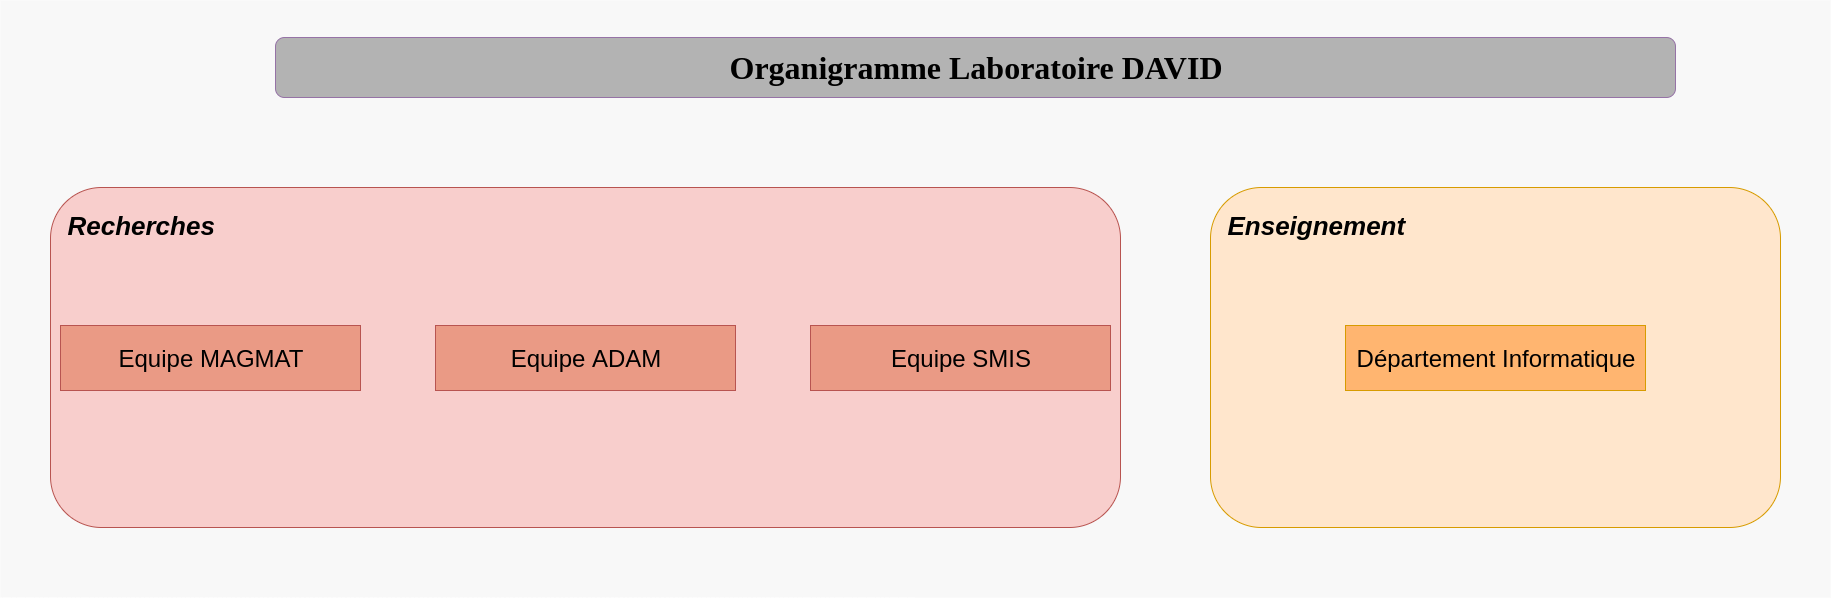
\includegraphics [width=10cm]{Organigramme_DAVID.png}
\end{textblock*}
\vspace{3cm}
 \begin{multicols}{2}
\begin{itemize}

\item Divis\'e en deux parties.
\item Plusieurs status diff\'erents.

\end{itemize}
\end{multicols}


\end{frame}
\end{subsection}

\begin{subsection}{L'\'equipe de travail}
\begin{frame}{L'\'equipe de travail}

\begin{itemize}
\item Travaille dans l'\'equipe MAGMAT.
\vspace{0,5cm}
\item Encadr\'e par:
\begin{itemize}
\vspace{0,30cm}
\item Yann STROZECKI.
\vspace{0,30cm}
\item Ma\"el GUIRAUD.
\vspace{0,30cm}
\item Joannes FALADE.
\end{itemize}
\end{itemize}


\end{frame}
\end{subsection}

\end{section}




\begin{section}{Pr\'esentation du travail accompli}

\begin{frame}
\tableofcontents[currentsection]
\end{frame}

\begin{frame}{Pr\'esentation du travail accompli}
\centering 
\includegraphics [width=25mm]{logos/logo_n-green.png}
\vspace{0,5cm}
\begin{itemize}
\item Projets de stage inscrits dans le projet N-GREEN.
\vspace{0,2cm}
\item Objectifs du projet N-GREEN:
\vspace{0,20cm}
\item Projet subventionn\'e par NOKIA BELL LABS.
\vspace{0,20cm}

\item Objectifs du stage:
\begin{itemize}
\item Visualisation du comportement d'un r\'eseau en anneau.
\item Simulation du r\'eseau avec diff\'erents param\`etres.
\end{itemize}
\end{itemize}

\end{frame}




\begin{subsection}{Les composants du r\'eseau}
\begin{frame}{Les composants du r\'eseau}


\begin{textblock*}{5cm}(36mm,1,1cm) % {block width} (coords)
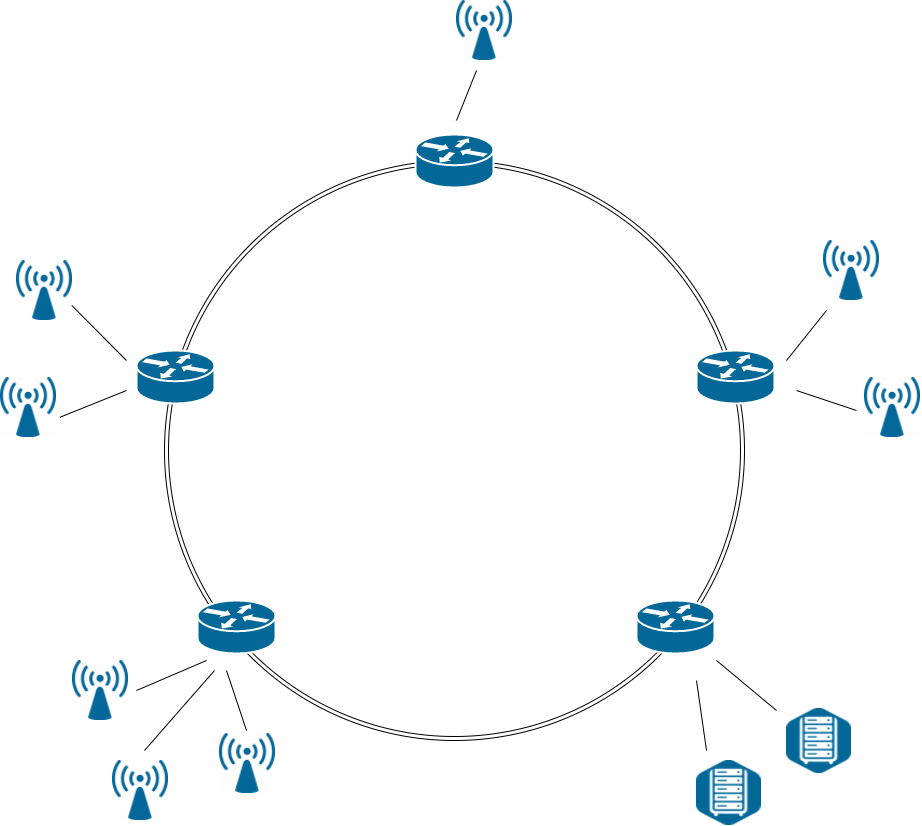
\includegraphics [width=5cm]{logos/anneau_N-GREEN.png}
\end{textblock*}


\vspace{3,5cm}

\begin{block}{Contexte g\'en\'eral}
 \begin{multicols}{2}
\begin{itemize}
\item Topologie du r\'eseau.
\item Centraliser les centres de calculs.

\end{itemize}
\end{multicols}
\end{block}

\end{frame}
 
 %%%FRAME AVANT HYPER EXPO
\begin{frame}{Mod\`ele}
\begin{textblock*}{5cm}(36mm,1,1cm) % {block width} (coords)
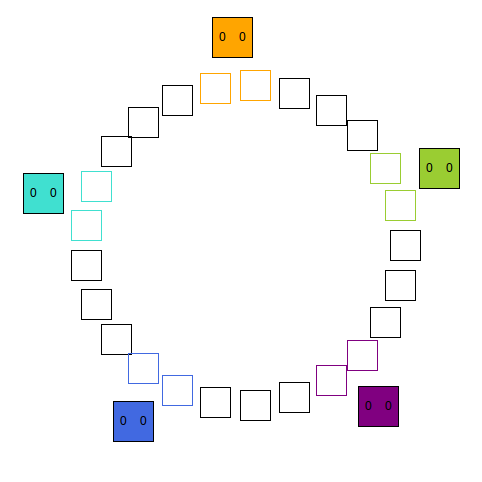
\includegraphics [width=5cm]{logos/anneau_en_action.png}
\end{textblock*}


\vspace{4cm}


\begin{textblock*}{5cm}(1cm,7cm) % {block width} (coords)

\begin{itemize}
\item Types de messages
\begin{itemize}
\item CRAN, prioritaires.
\item Best Effort, flux internet.
\end{itemize}

\end{itemize}

\end{textblock*}

\end{frame}

\begin{frame}{Hyper-exponentielle}
\begin{center}
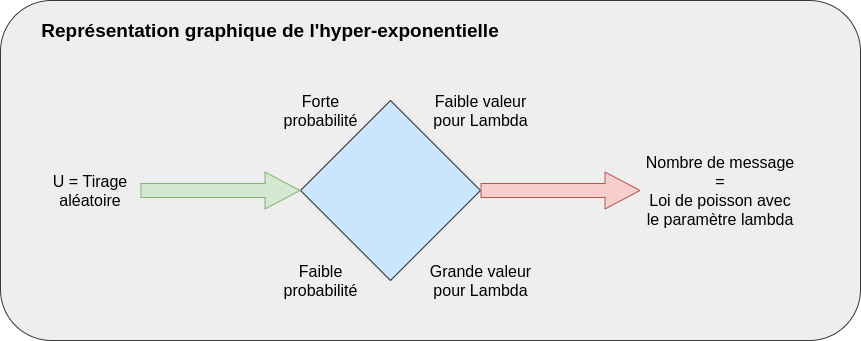
\includegraphics [width=100mm]{images/hyper_expo.png}
\end{center}
\end{frame}


%%%FRAME APRES HYPER EXPO
\begin{frame}{Mod\`ele}
\begin{textblock*}{5cm}(36mm,1,1cm) % {block width} (coords)
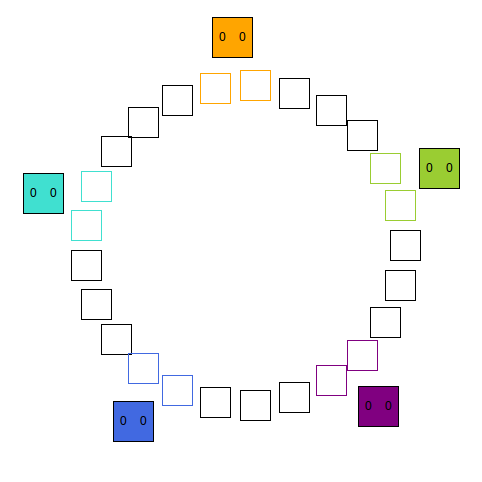
\includegraphics [width=5cm]{logos/anneau_en_action.png}
\end{textblock*}


\vspace{4cm}


 \begin{multicols}{2}
\begin{itemize}
\item Types de messages
\begin{itemize}
\item CRAN, prioritaires.
\item Best Effort, flux internet.
\end{itemize}
\item Politiques d'envoi:
\begin{itemize}
\item Stochastique.
\item Prioritaire.
\end{itemize}
\end{itemize}
\end{multicols}


\end{frame}



\end{subsection}


\begin{subsection}{Interface Graphique}
\begin{frame}{Interface Graphique}
 \begin{itemize}
 \item Objectif:
 \begin{itemize}
 \item Visualiser en temps r\'eel de l'\'etat de l'anneau: comportement selon diff\'erents param\`etres (nombre de noeuds, nombre de slots...).
  \end{itemize}
  \vspace{0,5cm}
\item Projet r\'ealis\'e en Python.
\vspace{0,7cm}
\item Utilisation du module graphique Tkinter.
  \end{itemize}
    \hspace{9cm} 
\includegraphics [width=20mm]{logos/logop.png}
\end{frame}


\end{subsection}


\begin{subsection}{Simulateur Statistique}
\begin{frame}{Simulateur Statistique}
 \begin{itemize}
 \item Objectif:
 \begin{itemize}
 \item G\'en\'erer des statistiques sur l'\'etat d'un anneau apr\`es une simulation sur un nombre d\'etermin\'e de TICs.
 \item Tester des politiques d'envoi des messages diff\'erentes.
  \end{itemize}
  \vspace{0,5cm}
\item Besoin de cr\'eer un programme rapide et optimis\'e:
 \begin{itemize}
 \item Langage C
 \item Graphiques g\'en\'er\'es par un script R.
 \item Optimisation du code.
   \end{itemize}
 \end{itemize}
 
 \begin{textblock*}{5cm}(8cm,6,5cm) % {block width} (coords)

\includegraphics [width=20mm]{logos/logor.png} 
\end{textblock*}

 \begin{textblock*}{5cm}(10cm,6,3cm) % {block width} (coords)
  
\includegraphics [width=20mm]{logos/logoc.png}
\end{textblock*}


\end{frame}



\begin{frame}{Politique Non-prioritaire}
\begin{center}
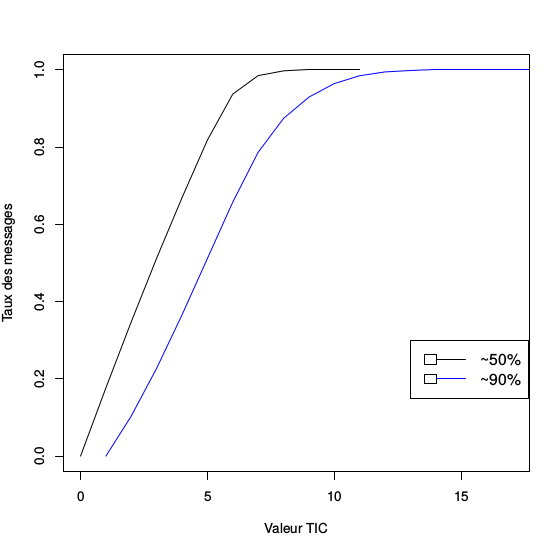
\includegraphics [width=60mm]{images/fonction_repartition_non_prioritaire.png}

Fonction de r\'epartition des temps d'attentes pour diff\'erentes charges (politique stochastique).
\end{center}
\end{frame}

\begin{frame}{Politique Prioritaire}
\begin{center}
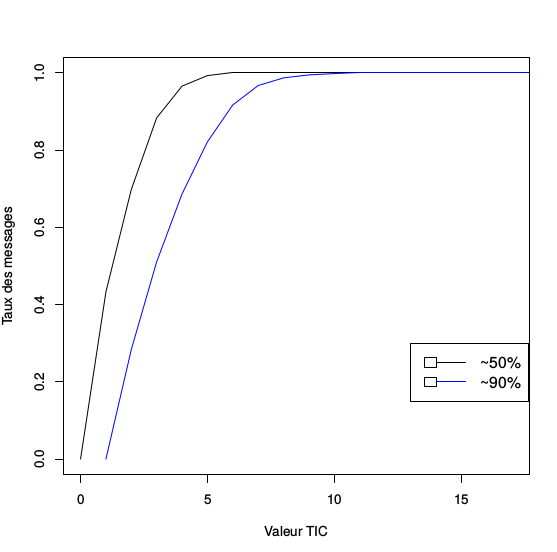
\includegraphics [width=60mm]{images/fonction_repartition_prioritaire.png}

Fonction de r\'epartition des temps d'attentes pour diff\'erentes charges (politique prioritaire).
\end{center}
\end{frame}
\end{subsection}



\end{section}

\begin{section}{Conclusion}

\begin{frame}{Bilan technique}
 \begin{multicols}{2}
\begin{itemize}
\item Utilisation des notions acquises pendant le DUT:
\begin{itemize}
\vspace{0,2cm}
\item Langages Python, R, C.
\item Utilisation des threads.
\item Organisation d'un projet.
\end{itemize}

\item Apprentissage et utilisation de nouveaux outils :
\begin{itemize}
\item Makefile
\item Valgrind
\item Tkinter
\end{itemize}

\end{itemize}

\end{multicols}
\end{frame}


\begin{frame}{Conclusion}

\begin{itemize}
\item Visualisation et simulations de diff\'erentes politiques d'envoi des messages dans l'anneau.
\item Analyse statistique des r\'esultats
\vspace{1cm}
\item {\bf Confirmation de ma volont\'e de r\'ealiser un th\`ese et de travailler en laboratoire.}

\end{itemize}
\vspace{1cm}
 \centering
  
\includegraphics [width=15mm]{logod.png} \hspace{1,5cm} 
\includegraphics [width=20mm]{logon.png} \hspace{1cm} 
\includegraphics [width=25mm]{logos/logo_iut.jpg} \\
\end{frame}


\begin{frame}{Merci de votre attention}
\begin{center}
  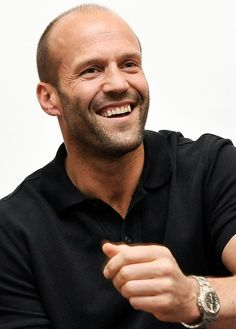
\includegraphics [width=30mm]{logos/jason.jpg}
 \begin{textblock*}{5cm}(4cm,8cm) % {block width} (coords)
  Merci de votre attention!!
  \end{textblock*}
  \end{center}
\end{frame}


\end{section}





\end{document}
